\section{Kubernetes distribution}
Dalam penelitian ini akan dibahas tiga distribusi kubernetes yaitu KubeEdge, MicroK8s, serta K3s. Masing masing dari distribusi ini memiliki kegunaan dan fungsi nya masing masing. Walaupun semuanya memiliki \textit{support} untuk IoT namun setiap distribusi memiliki cara unik tersendiri untuk menyelesaikan masalahnya.

\subsection{KubeEdge}
KubeEdge merupakan solusi \textit{edge architecture} \textit{open source} yang mengembangkan kubernetes secara lebih jauh untuk domain spesifik yaitu \textit{IoT} \parencite{kubeedge}. Arsitektur KubeEdge memungkinkan untuk melakukan konfigurasi perangkat \textit{IoT} yang berada di \textit{edge} secara terpusat melalui komponen \textit{cloud}. Dengan adanya dua komponen \textit{edge core} dan \textit{cloud core} membuat komunikasi antara platform aplikasi menjadi \textit{seamless}.

Untuk menghubungkan \textit{cloud core} dengan \textit{edge core}, KubeEdge menggunakan sebuah \textit{controller} yang dapat melakukan \textit{device discovery} terhadap \textit{edge core}. Setelah \textit{edge core} ditemukan, \textit{controller} akan meneruskan \textit{request} ke komponen berikutnya yaitu Sync Service. KubeEdge menggunakan KubeBus untuk melakukan komunikasi antar \textit{cloud} dan \textit{edge}, KubeBus menggunakan protokol HTTP untuk meneruskan \textit{request} dari \textit{cloud core} menuju \textit{edge core}. Setelah \textit{request} diterima oleh \textit{edge core}, akan digunakan protokol MQTT untuk menerima ataupun mengirim data dari perangkat \textit{IoT} ke \textit{edge core} begitu pula sebaliknya.

\begin{figure}[h]
  \centering
  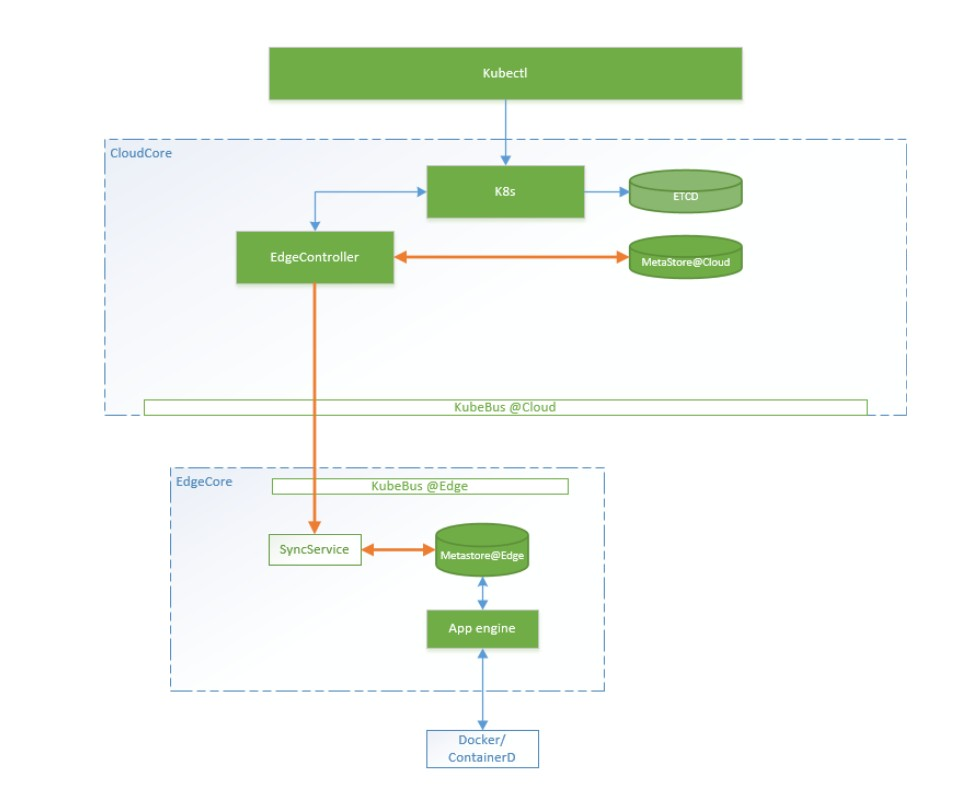
\includegraphics[width=1\textwidth]{resources/chapter-2/arsitektur-kube-edge.jpg}
  \caption{Arsitektur KubeEdge \parencite{kubeedge}}
  \label{fig:arsitektur-kube-edge}
\end{figure}

\subsection{Microk8s}
MicroK8s adalah sebuah platform \textit{open-source} yang digunakan untuk mengotomatisasi distribusi, \textit{scaling}, dan manajemen aplikasi yang berbasis kontainer. MicroK8s menyediakan fungsionalitas inti pada Kubernetes, dengan ukuran yang kecil, dan dapat di-\textit{scale} dari satu node hingga menjadi cluster produksi yang yang besar \parencite{microk8s}.

Dengan mengurangi penggunaan sumber daya yang dibutuhkan untuk menjalankan Kubernetes, MicroK8s memungkinkan penggunaan Kubernetes dalam berbagai lingkungan, seperti:

\begin{enumerate}
  \item Mengubah Kubernetes menjadi alat pengembangan yang ringan.
  \item Menjadikan Kubernetes tersedia untuk digunakan dalam lingkungan minimal seperti GitHub CI (Continuous Integration).
  \item Menyesuaikan Kubernetes untuk aplikasi IoT pada perangkat dengan \textit{resource} yang terbatas.
\end{enumerate}


\subsection{K3s}
K3s adalah sebuah platform \textit{open-source} yang memfasilitasi penggunaan Kubernetes dengan ukuran yang lebih ringan dan mudah diimplementasikan. K3s dikembangkan untuk memudahkan distirbusi dan manajemen Kubernetes dalam lingkungan yang lebih sederhana dan bersifat minimalis. K3s dibuat untuk mendukung pengembangan pada ranah \textit{IoT} karena K3s memiliki support sepenuhnya untuk arsitektur ARM serta cocok untuk digunakan pada lingkungan edge dan \textit{IoT} \parencite{k3s}.

K3s memiliki dua komponen utama yaitu \textit{server, agent}. \textit{Server} dapat dikatakan sebagai sebuah \textit{control plane} atau \textit{master node} yang digunakan pada K3s berfungsi untuk mengatur seluruh permintaan ataupun request dari \textit{agent}. \textit{Server} memiliki tanggung jawab penuh terhadap masing masing \textit{agent} yang terhubung mulai dari menyimpan data dari masing masing \textit{agent}, \textit{controller}, serta \textit{scheduler} \parencite{k3s}. \textit{Agent} di sisi lain berfungsi sebagai \textit{slave node} yang akan mengeksekusi semua perintah dari \textit{server} atau \textit{master node}. 

\begin{figure}[hb]
  \centering
  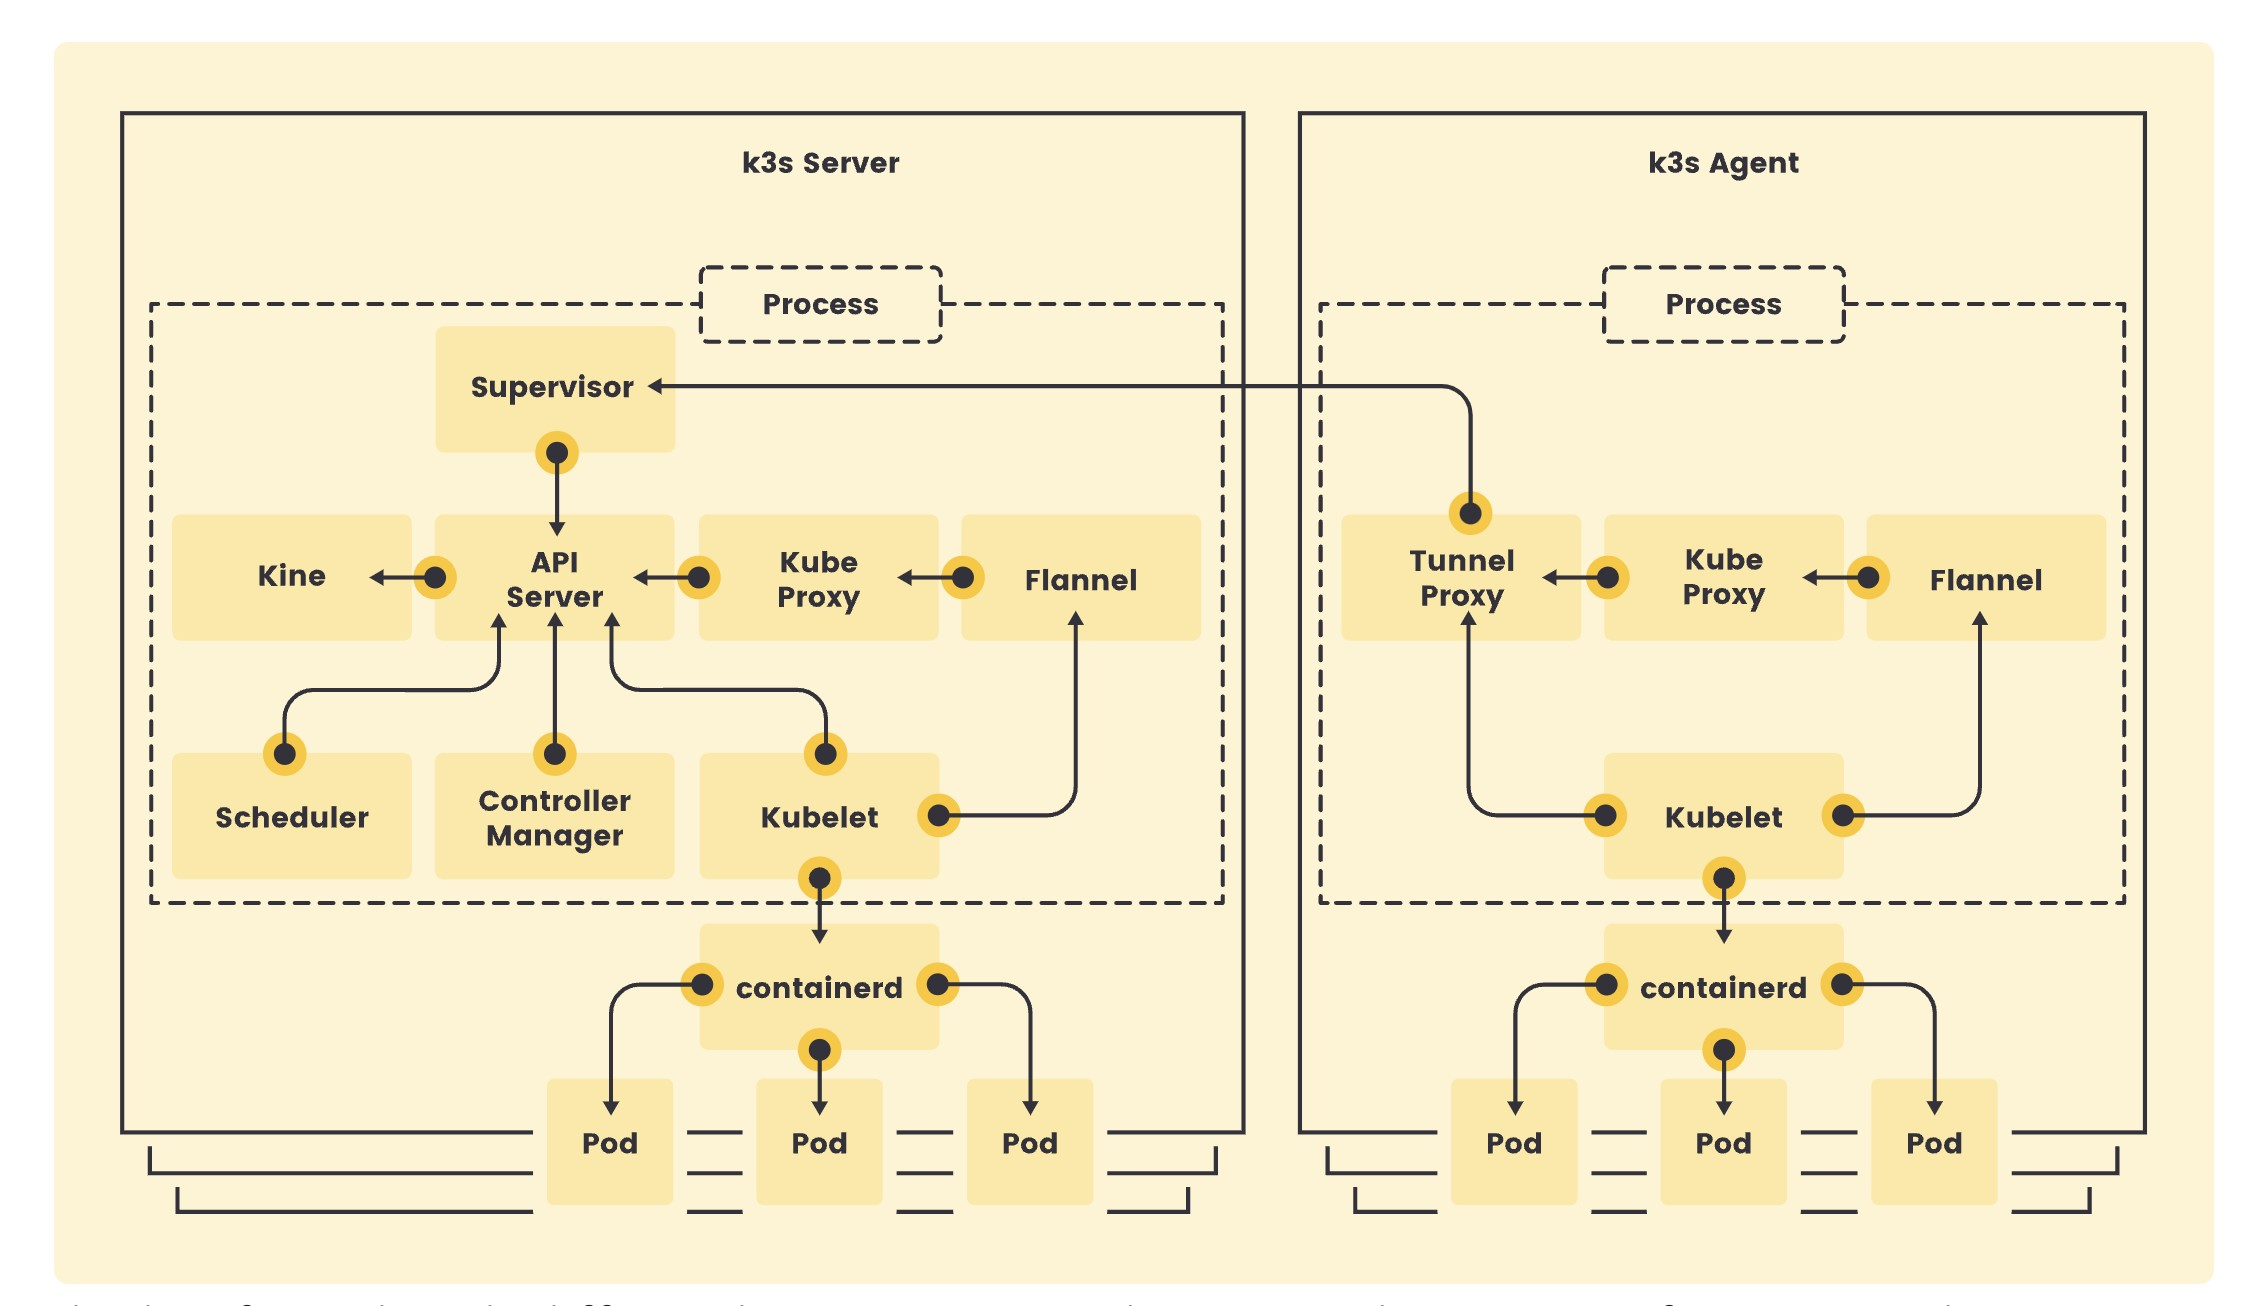
\includegraphics[width=1\textwidth]{resources/chapter-2/arsitektur-k3s.jpg}
  \caption{Arsitektur k3s \parencite{k3s}}
  \label{fig:arsitektur-k3s}
\end{figure}
